%% LaTeX2e class for student theses
%% sections/content.tex
%% 
%% Karlsruhe Institute of Technology
%% Institute for Program Structures and Data Organization
%% Chair for Software Design and Quality (SDQ)
%%
%% Dr.-Ing. Erik Burger
%% burger@kit.edu
%%
%% Version 1.4, 2023-06-19

\chapter{Security Analysis}
\label{Security Analysis}

This chapter contains an overview of threats and how, if so, TDX protects against them. This analysis is by no means comprehensive, but meant as an overview. It gives examples of real attacks using the aforementioned attack vectors. In addition ways to establish a secure connection to a TD and TD identity verification are discussed.

\section{Already known attacks and vulnerabilities}

This section gives examples of attacks inside and outside the threat model that have already been proven to be effective against either SGX or TDX. The line what is inside the Threat model and what is outside can sometimes be vague, especially in regards to physical attacks. In \cref{Threat_Model} I have already tried to clear this up and this section will explain some attacks that can break TDX.

As described in \cref{Threat_Model} TDX considers the cloud provider, with physical access, as untrusted. This means that any physical attack should be defended against, but as outlined previously this is not the case. Opening the case does not provide a significant hurdle for any attacker, who already has physical access. This leaves TDX vulnerable to any sort of attack that can be executed with physical hardware access, that can break SGX. This includes Plundervolt which can break the integrity and indirectly the confidentiality of SGX \cite{munoz_survey_2023}, which is, as outlined in \cref{TDX Architecture} relied upon for TDX. Platypus attack which was also shown to break the integrity of SGX \cite{Lipp2021Platypus} and more \cite{lipp_nethammer_2018} \cite{tang_clkscrew_nodate}. While attacking a specific TD inside a data center is non-trivial it is not impossible. This means that as long as hardware access is not prevented completely TDX can not prevent access to data inside the TD. TDX can by their very nature not protect against all side-channel attacks. It protects against some well known ones such as the spectre-family. TDX does not have mitigations to address memory access patterns as it just uses encrypted memory. Privacy leakage from memory access attacks was already shown to take less than a couple of minutes on consumer grade hardware. John et Al. were able to infer a 512-bit secret in just three and a half minutes only using write-access patterns \cite{john_connecting_2017}.



\section{Connecting to the correct TD}

This section explains how to verify a TDs identity and then how to securely connect to this TD. Without verifying the TDs identity a secure connection can not be established, because the endpoint is not verified.

\myparagraph{Verifying the TD identity}

\label{Identity}
Similarly to SGX, with TDX the quote contains information on the startup environment of the TD. The Measurement of Trust Domain (MRTD) registers contain information on the initial state of the TD immediately after startup. Its calculation is based on the page content during startup \cite{intel_corporation_dcap_2024-1}. The Runtime Measurement Registers (RTMR) are written during runtime, Intel recommends writing information about the virtual firmware configuration in RTMR[0] and information about the OS kernel and boot parameters or more importantly kernel parameters in RTMR[1]. Information about these can be supplied by the virtual firmware, which is written by Intel and should thus follow their own recommendations. It is unclear these are written. They are either filled after startup by the TDVF \cite{intel_corporation_tdx-virtual-firmware-design-guide-rev-004-20231206pdf_2023}, somehow supplied by the host, although this would make them untrusted and worthless, written after the TD requests the TDX Module to do so \cite{intel_corporation_tdx-virtual-firmware-design-guide-rev-004-20231206pdf_2023} or just filled by the TD itself \cite{noauthor_tdx-module-10-public-specpdf_nodate}. Testing later shows that they are empty immediately after startup on an Azure VM.
RTMR[2] is used as a replacement for the Platform Configuration Register from TPM, to hold the aggregate integrity value of the IMA runtime measurement list. To do this Intel had to introduce an additional kernel driver and an update for IMA \cite{haidong_xia_runtime_integrity_measurement_2024}. The IMA update has not been made public on the official IMA repository at \url{https://sourceforge.net/projects/linux-ima/} as of yet. In the future Intel wants to support a virtualized version of TPM, so that an unaltered Kernel can be used. To ensure traceability the event logs related to the list of measurements will be kept in the Confidential Computing Event Log (CCEL) table \cite{haidong_xia_runtime_integrity_measurement_2024}. The CCEL is created during startup and rooted inside the UEFI reserved memory. The User can use either /dev/mem or /sys/firmware/acpi/tables/data/CCEL, which is read-only, to access the data inside it. Many systems have /dev/mem disabled for security reason, that is why the additional firmware table was added.

\subsection{Establishing a secure connection to the TD}

This section proposes three different ways to establish a secure connection. They are sorted in order of increasing complexity.

\label{Establishing_a_secure_connection}

\myparagraph{Simple SSH connection to a TD}

\label{SSHConnection}
Prior to TD creation the image can be build containing a known user public ssh key. If it is the only key present and password authentication is deactivated, the TD will decline connection attempts by anyone without the corresponding private key. This is generally how cloud providers provide VMs. This being the only key present can be verified via measurements in the TD Quote as discussed previously. If possible the startup measurements should be compared to a selfbuild image containing just the users public key, if not possible the TD identity can not be verified and no secure connection can be established. The TD has to put its own public key into the REPORTDATA field of its quote so the user can then verify its fingerprint when establishing a connection. This connection is vulnerable during the first connection as it is unsecured. No sensitive data should thus be transmitted before the quote is not received and verified. After verifying the TD identity and getting its public SSH key, a new connection has to be established. If the user is the only person being able to access this specific TD then this means that it is no longer possible to fake the man-in-the-middle attack in Figure \ref{fig:man_in_the_middle} because the attacker would not have access to a TD that can create the correct quote. This form of secure communication relies on the fact that only one public key is in the TD. It also depends on the user to verify the TDs identity upon connecting and also for subsequent connection attempts that the fingerprint of the TDs cannot be recreated for transcript collision attacks \cite{bhargavan_transcript_2016}.

\myparagraph{TLS connection to a TD}

According to Cheng et Al. TDX and SGX can establish secure channels via TLS in a similar way \cite{cheng_intel_2023}:
In a typical scenario, when a client negotiates a secure channel with a server running in a TD, it aims to ensure a connection with a server that has been properly instantiated. The server, acting as an attester, generates a pair of ephemeral public and private keys. It calculates the hash of the public key, creates a TD quote with its key inside the REPORTDATA and generates a self-signed certificate with the quote embedded in it. This self-signed certificate is provided as the server certificate in the TLS handshake protocol. Upon receiving the server certificate, the client, acting as the challenger, verifies the signatures on the certificate and validates the embedded quote, including the measurements. The client also checks if the quote includes the hash of the public key, as this associates the key with the TD. This contains the assumption that the client can verify the TD identity from the Quote, which is not given. When establishing a secure channel, both the client and server can assume the roles of attester and verifier. This enables endpoints running in TDs to authenticate each other mutually by validating TDs. Issues arising from self-signed certificates, the certificate size and similar are all discussed as well by Knauth et Al., with all of them having solutions \cite{knauth_integrating_2019}. Although the latter can mean that the entire TD can be compromised which invalidates other security assumptions. Therefore this variant and the SSH connection have similar security assumptions and guarantees.
Lastly an add-on to the previous method of establishing a secure connection is the usage of a complete application in the image, that does only expose certain endpoints to the web. Using proper authorisation against those endpoints, makes unwarranted access impossible. Additionally, having the application immediately on startup create the necessary certificate from the previous paragraph, prevents attacks on the initial connection as well. This is Intels recommended way of using TDX and starting a TD. 

\myparagraph{Using Initramfs and encrypted disk images}

Using a custom Kernel with a custom Initramfs that mounts an encrypted disk and contains TDX attestation capabilities as well as a predetermined public user SSH key, it is possible to establish a secure connection as well. Intel recommends implementing these capabilities in their Guest to Hypervisor communication Interface specifications aswell \cite{intel_corporation_guest_hypervisor}. This relies on the same mechanisms as \ref{SSHConnection} but gives the additional benefit, of containing an encrypted storage volume. It can thus safeguard sensitive data inside the image from unauthorized access. Upon startup the TD will pause the start after the Kernel has been loaded. The Initramfs will be loaded and active here as well. The challenger can now use its private key to the public ssh key inside the Initramfs to establish a secure connection. The challenger can now create a TD quote containing the Kernel measurements. Verifying the kernel measurements inside the TD quote and can then supply the key to the encrypted disk image to continue booting. According to Intel it should be possible to safe the encryption key inside the memory using the Storage-Volume-Key-Location ACPI Table \cite{intel_corporation_guest_hypervisor}. Intel even recommends usage of these tables in their design guide \cite{intel_corporation_guest_hypervisor}. They do not explain how these could be adequately protected from unauthorized access by, for example, the cloud provider. If disk encryption is used, dm-crypt provides the ability to use disk encryption with authentication. It is now guaranteed that the image inside the encrypted disk image is now executed only once and is running inside a TD. Choosing a secure channel to this TD depends on the code inside. Having an additional SSH key inside, as explained previously, can work.

\section{Attestation Verification}

There are generally four ways how attestation can be done that have their pros and cons. They are outlined in \cref{tab:AttestationVerification}. Intel is considered an independent vendor in this comparison as they are independent from the cloud provider that is in question. Intel is also already a trusted party, at least in terms of their hardware, and more importantly all attestation verification services have to at least talk to Intels provisioning certification service.

\begin{table}
\centering
\resizebox{0.9\textwidth}{!}{%
\begin{tabular}{ m{0.3\textwidth} m{0.2\textwidth} m{0.2\textwidth} m{0.2\textwidth} m{0.2\textwidth}}
\toprule
& Cloud Provider Attestation Service & Application Vendor Attestation Service & Third Party Trust Service (E.g. Intel Trust Authority) & Build-Your-Own Service with DCAP \\
\midrule
Seperation of responsibilities between verifier and infrastructure provider & No & Yes & Yes & Yes \\
\midrule
Consistency across SGX and TDX & Yes, if both are offered & Yes, if both are supported & Yes & Yes \\
\midrule
Consistent service across on-prem, hybrid, multi-cloud, and edge deployments & No & Possible but unlikely or limited & Yes & Yes\\
\midrule
Development Effort & Low & Low & Low & Medium \\
\bottomrule
\end{tabular}
}
\caption{Overview of four different Attestation Verification methods}
\label{tab:AttestationVerification}
\end{table}
This thesis will focus on Cloud Provider Attestation Service, and more specifically Microsoft Azure Attesation (MAA). The security assumptions and guarantees for this will then be compared to a Build-Your-Own Service using DCAP. MAA also has to use Intels DCAP to generate and verify quotes. 

\subsection{Cloud Provider Attestation Service}
 Microsoft, offers an attestation verification service hosted and implemented by them. They also offer an implementation of Intel DCAP to generate a quote. This can then be automatically verified via MAA or Intel Trust Authority or manually using your own DCAP implementation. Intel Trust Authority was not available for testing.

\myparagraph{Microsoft Azure Attestation}

This section will explain in detail how MAA can be used, the pitfalls for the user, and any other issues with it that were found. First to use MAA, one has to create a confidential VM with Azure. Microsoft provides a tutorial to create a TD VM \cite{chasecrum_github_create_2024}, which does not create a TD, that has the characteristics discussed in \cref{TDX Architecture}. The Issues with the TD used as well as the firmware are explored at the end of this section. Following the instructions provided by Azure, it is also not explained how to choose between AMD SEV-SNP and Intel TDX. This decision is entirely up to the chosen VM size which can only be inferred by looking at press releases pertaining to Intel TDX and the newly released VM sizes. The DC\textbf{e}sv5, DC\textbf{e}dsv5 and EC\textbf{e}sv5, EC\textbf{e}dsv5 use Intel Xeon CPUs, while DC\textbf{a}sv5, DC\textbf{a}dsv5 and EC\textbf{a}sv5, EC\textbf{a}dsv5 use AMD Threadripper CPUs. The difference between D-instances and E-instances is the ratio between VCPU cores and memory, with E-instances having more memory per core. With the VM created there are a couple of ways to create a TD Quote for attestation: Using an Intel-supplied or a self-written implementation of Intel DCAP and the Azure confidential-computing-cvm-guest-attestation library \cite{microsoft_corporation_azureconfidential-computing-cvm-guest-attestation_nodate}. Building the tdx-attestation app and using the supplied maa\_config file, which does only contain three settings, succeeds in creating a TD quote and then returns a JSON Web Token from the Microsoft Azure attestation Service. A complete example token can be found in \cref{jwt} but here we will focus on some parts of the td quote body. Intel has already given short explanations for all TDX registers \cite{intel_corporation_dcap_2024-1}, which will be explained further. We know that this has to be TDX 1.5 because tdx\_mrseam is not filled with 0, which would indicate TDX 1.0. The TEE\_TCB\_INFO struct contains two measurements, which are expected to be non-zero: MRSEAM, which is the measurement of the TDX Module and TEE\_TCB\_SVN, which contains the security version number of the TCB inside the TDXM, one that has to be 0 with TDX: MRSIGNERSEAM, which is a relict from SGX and one that can be either: TD\_ATTRIBUTES, this contains flags for the debugmode and future reserved flags. These all fit the expectation. Intels recommendation for runtime-measurement registers tdx\_rtmr0 and tdx\_rtmr1 are as follows: RTMR0 stores the measurements for TD Virtual Firmware, these are influenced by tdvm launch parameters, such as memory size. Most importantly this is locked in during startup and thus not user controlled in a cloud environment, although those can be overwritten, those changes would be loggend in the ACPI CC log table \cite{uefi_forum_inc_acpi_docu_2022}. In the excerpt returned by MAA this is filled with 0. RTMR1 should have two different purposes, depending on the boot option for the VM. With a direct boot it stores the kernel measurements and cmdline, that is passed to the kernel. With a grub boot it stores the grub measurements \cite{intel_corporation_tdx-virtual-firmware-design-guide-rev-004-20231206pdf_2023}. Those measurements should be written during startup and their changelog should also be written in the CC-Event log table. The register returned by MAA is once again only filled with 0, which goes against the recommendations of Intel. The virtual firmware Intel offers for use does follow these instructions, meaning the firmware in use is a custom one by Microsoft which overwrites these best-practices. MRTD contains measurements, which include the virtual firmware, it can thus be used to verify the firmware in use. Especially RTMR1 with its Kernel measurements is invaluable to the identity verification measurements provided in \cref{Identity}.
\begin{lstlisting}[language=jsonmain,caption={TDX generated part of an MAA quote},captionpos=b]
  "tdx_mrconfigid": "000000000000000000000000000000000000000000000000000000000000000000000000000000000000000000000000",
  "tdx_mrowner": "000000000000000000000000000000000000000000000000000000000000000000000000000000000000000000000000",
  "tdx_mrownerconfig": "000000000000000000000000000000000000000000000000000000000000000000000000000000000000000000000000",
  "tdx_mrseam": "360304d34a16aace0a18e09ad2d07d2b9fd3c174378e5bf108388079827f89ff62acc5f8c473dd40706324834e202946",
  "tdx_mrsignerseam": "000000000000000000000000000000000000000000000000000000000000000000000000000000000000000000000000",
  "tdx_mrtd": "024a32b070383331181619fa387cb4d55d1e38879f989933055ccad5bc2db795d1737b66205949d15469dc8c1ba7ab7b",
  "tdx_report_data": "c90f98ba8ab80c7b442b6b8eb30af54e0508077b11adb525af6dfbcc8714e52a0000000000000000000000000000000000000000000000000000000000000000",
  "tdx_rtmr0": "000000000000000000000000000000000000000000000000000000000000000000000000000000000000000000000000",
  "tdx_rtmr1": "000000000000000000000000000000000000000000000000000000000000000000000000000000000000000000000000",
  "tdx_rtmr2": "000000000000000000000000000000000000000000000000000000000000000000000000000000000000000000000000",
  "tdx_rtmr3": "000000000000000000000000000000000000000000000000000000000000000000000000000000000000000000000000",
  "tdx_seam_attributes": "0000000000000000",
  "tdx_seamsvn": 258,
  "tdx_td_attributes": "0000000000000000",
  "tdx_td_attributes_debug": false,
  "tdx_td_attributes_key_locker": false,
  "tdx_td_attributes_perfmon": false,
  "tdx_td_attributes_protection_keys": false,
  "tdx_td_attributes_septve_disable": false,
  "tdx_tee_tcb_svn": "02010600000000000000000000000000",
  "tdx_xfam": "e718060000000000"
\end{lstlisting}
\label{td_quote}

\myparagraph{Issues with the Image and Firmware used in the Azure TD}

\label{Issues-with-azure-td}
Intel recommends testing for three different things as the first step of identifying a TD, although they themselves are not sufficient to proof the presence of a TD and could theoretically be faked. In the file /proc/cpuinfo there needs to be a flag for tdx\_guest, this did not exist. The CC Event Log ACPI Table needs to contain CC Type 2 for TDX - this table was not even present, which is contrary to efi best practices \cite{uefi_forum_inc_acpi_docu_2022}. /dev/mem was also not accessible. Information from this table are also necessary for TD validation in general. This information should also have been present in the rtmr0 register. Lastly a character device called tdx\_guest, tdx-attestation or tdx-guest depending on the version should be present. These function as an interface to retrieve TDX guest specific information from the TDX Module \cite{linux_kernel_development_community_tdx_2024}. It is used to retrieve the TDREPORT for the attestation, covering steps 2 and 8 in Fig\ref{fig:QuoteGeneration}. This was also not present. This means that the guest VM was not a TDX enlightened guest VM as discussed previously in \cref{TDX Architecture}, nor is it compliant with other confidential computing VM standards. This itself does not make the cvm hardware attestation impossible, but makes it much more difficult to implement your own attestation and also verify if the cvm is correct. It appears that Microsoft recreated the tdx\_guest interface somewhere but does not tell the user how it was done, if it was done exactly the same way or how to use it themselves. The User needs to somehow recreate the functionality of this character device manually if they want to implement their own attestation. All of these changes go against the recommendations by the EFI specifications as well as Intels recommendations for TD implementations.
The tdx\_guest interface is also used to write the runtime measurements into the registers, which is now not possible. Thus those are filled with 0 in \cref{td_quote}. It should also be possible to add custom REPORTDATA, for example a nonce or any additional data to the quote. Adding this to the guest-attestation implementation does not change the resulting quote.
Looking further into the implementation of the cvm-guest-attestation tdx implementation, they support measurements via something called TCGLog, which appears to be a windows-only implementation of the \guillemotright TCG measured boot logs \guillemotleft \cite{graeber_mattifestationtcglogtools_2023} from the Trusted Computing Group. As of now it is thus not possible to create a TD Quote with any kind of measurement in the Azure Cloud. 
Verifying MAAs implementation is not possible as \guillemotright"Source code is [only] available for government customers via the Microsoft Code Center Premium Tool \guillemotleft \cite{dan_mabee_azure_attestation_2023}. It is not possible to supply your own image and the provided images by Azure do not have public hashes. Using the TDX IMA integration discussed in \ref{Identity} is also not possible with Azure in general.
The Azure attestation token is signed with a self-signed certificate, which was retrieved from \url{https://attestationprovidername.attest.azure.net/certs}, the signature does match. The same certificates contains the SGX quote from the azure attestation enclave, which was verified via the valid implementation of DCAP located at \cite{microsoft_corporation_azure-samplesmicrosoft-azure-attestation_nodate}. This confirms just that azure attestation runs inside a functioning SGX enclave. Additionally it is possible to validate the binding of the azure attestation SGX key with the key that signed the attestation token via the hash of the public key in the reportdata field of the quote.

\section{Security Summary}

The literature has shown that TDX predecessor SGX was vulnerable to many attacks and vulnerabilities, inside its threat model. Some of these issues were fixed by Intel and some had to be fixed by the application developer themselves. If we assume that TDX can completely protect against all attacks inside its threat model, the distinction between basic and complex physical attacks is rather important. Intel stated that opening the case to access the hardware directly constitutes an attack outside its threat model and thus a complex physical attack. This means anyone with hardware access, who can open a case can potentially attack and compromise a TD. This includes the cloud provider, who Intel wanted to exclude from the list of trusted parties explicitly.
Going further into actually using a TD on Microsoft Azure, it was shown that the Cloud Provider has to still cooperate, while it can be shown, if they do not do so completely, this does not give additional security guarantees. It is possible and plausible that the Quote created by Azure is genuine and comes from the TD, that was created for this thesis, it could not be proven.

\chapter{Performance Analysis}

\label{performance}

\section{Setting up a TDX VM on a new machine}
\label{ch:SettingUpTDX}
Intel supplies documents for a quick setup of TDX machines and TDs. In this section, Intels Whitepaper for its Linux Stack for Intel TDX will be used as a reference \cite{noauthor_white_nodate}. Intel internally supplies additional documents as well and code from there will be replicated here if possible. The Server was supplied as an Intel DevCloud bare-metal machine with two Intel XEON 8490h processors with 60 cores respectively. Setting up Intel DevCloud and Trusted Domain for the first time took the better part of a week. The versioning in the different internal guides was off, which lead to an unusable kernel, which was only fixed by complete reinstall. The TDX-tool version used in the end was 2023ww22 from may 2023, which can be found on the tdx-tools Github \cite{intel_corporation_inteltdx-tools_2024}. The guest image was created using the guest image creation tool. The entire BOM can be found in \cref{tab:BOM}

\begin{table}
\centering
\resizebox{\textwidth}{!}{%
\begin{tabular}{ {0.15\textwidth} m{0.2\textwidth} m{0.2\textwidth} m{0.2\textwidth} m{0.2\textwidth} m{0.2\textwidth} m{0.2\textwidth} m{0.2\textwidth}}
\toprule
Component & Kernel & Libvirt & QEMU & Grub2 & OVMF & Shim & amber-cli \\
\midrule
Ubuntu Version & 5.19.17-mvp23v3+6 & 8.6.0-2022.11.17.mvp1 & 7.0.50+mvp9+15 & 2.06-mvp3 & 2023.03.07-stable202302.mvp9 & 15.4-mvp3 & 2023ww21-mvp3 \\
\bottomrule
\end{tabular}
}
\caption{Comparison of different timings of IPEX optimization method}
\label{tab:BOM}
\end{table}
The tdx-tools installs all the necessary kernel components to the images, as well as checking the respective hashes. Next the host kernel has to be patched. This requires downloading the correct packages from the Intel open source directory and then creating a patched kernel. Next TDX can be enabled and booted up using the newly patched kernel. To enable the possibility of attestation, the kernel needs Intel SGX DCAP, which can also be installed from the Intel open source directory or downloaded from Github. Additionally an implementation of the Provisioning Certification Caching Service, which Intel provides a reference implementation of, is also needed. This implementation can also be found in the Intel open source directory. Lastly, the Quote Generation Service contained in the SGX SDK must be installed. Now the Guest TD can be booted up using QEMU with the following command:
\begin{lstlisting}[language=json, frame=single, float=h,caption={test}]
     /usr/bin/qemu-system-x86_64 -accel kvm -name process=tdxvm,debug-threads=on -m 64G -vga none -monitor pty -no-hpet -nodefaults -drive file=/tmp/tdx-guest-ubuntu-22.04.qcow2,if=virtio,format=qcow2 -monitor telnet:127.0.0.1:9001,server,nowait -bios /usr/share/qemu/OVMF.fd -object tdx-guest,sept-ve-disable=on,id=tdx -object memory-backend-memfd-private,id=ram1,size=64G -cpu host,-kvm-steal-time,pmu=off -machine q35,kernel_irqchip=split,confidential-guest-support=tdx,memory-backend=ram1 -device virtio-net-pci,netdev=mynet0 -netdev user,id=mynet0,net=10.0.2.0/24,dhcpstart=10.0.2.15,hostfwd=tcp::10026-:22 -smp 32 -chardev stdio,id=mux,mux=on,logfile=/home/test/tdx-tools/vm_log_2024-03-08T0901.log -device virtio-serial,romfile= -device virtconsole,chardev=mux -monitor chardev:mux -serial chardev:mux -nographic
\end{lstlisting}

\section{Benchmarks}

This section will explain how the benchmarks were setup and executed and then discuss their results.

\subsection{Setting up the benchmarks}
\label{sec:SecondContent:SecondSection}

The benchmark will be run in Python, as it is the most commonly used programming language in natural language processing. The benchmarks will predominantly be an inference benchmark using distillBERT and roBERTa-base. These two were chosen as they already had support for Intel AMX. They are both part of the BERT family of Large Language Models, which offer already useful language inference without additional modification \cite{devlin_bert_2019}. All benchmarks will be run using the same image on their own QEMU KVM with 32 Cores and 64GB of RAM, except if stated otherwise. Performance is measured with Pyperf and each test is run 30 times with the median and the standard deviation being shown.
For the inference Benchmark a short sentence with 16 tokens and a long passage with 146 tokens, according to the BERT tokenizer were used. The long passage was supposed to have 128 tokens but due to an oversight the passage was a bit longer than initially thought. The sentences and their corresponding arrays can be seen in the following listing:
    \begin{minted}[breaklines,frame=single]{python}
    sentence_short = "The sun sets, painting the sky with hues of orange and pink"
    sentence_short_array = [sentence_short] * 8
    
    sentence_long = "In the heart of the city, amidst the bustling streets, lies a hidden gem—a café tucked away from the chaos of urban life. Inside, the aroma of freshly brewed coffee mingles with the scent of baked goods, enticing passersby to step in and indulge their senses. Jazz music fills the air, creating a cozy atmosphere that invites patrons to linger a little longer. The café buzzes with activity as people chat over steaming cups of espresso or lose themselves in the pages of a good book. Outside, the world rushes by, but within the café's walls, time seems to slow down, offering a moment of tranquility amidst the frenzy of the city."
    sentence_long_array = [sentence_long] * 8
    \end{minted}

    Before each benchmark a short warmup of 100 iterations was run. Then the pyperf benchmark function with 5 inner loops was called. This was then repeated for all eight benchmarks per model.
    
    \begin{minted}[breaklines,frame=single]{python}
    runner = pyperf.Runner()
    def warmup(pipeline, data):
        for i in range(100):
            result = pipeline(data)
    def bench(pipeline, data, iterations):
        for i in range(iterations):
            result = pipeline(data)
    warmup(pipe, sentence_short)
    runner.bench_func(f"Transformer pipe, short sentence, {model}", bench, pipe, sentence_short, 100, inner_loops=5)
    \end{minted}
    


\subsection{Benchmark and data evaluation methods}

In this thesis in general the Median Absolute Deviation opposed to the standard deviation will be used to compare different results. While the standard deviation (std dev) is the de facto standard in the field of statistics it does not need to be \cite{gorard_revisiting_2005}. The main benefit of the standard deviation was in the past its ease of calculation and when drawing from normal-distributed populations \guillemotright the standard deviation of their individual mean deviations is 14\% higher than the standard deviations of their individual standard deviations. \guillemotleft \cite{gorard_revisiting_2005}
With most results, it is generally expected to get something along a normal distribution but this assumption does not appear to be correct with memory benchmarks according to Lemire \url{https://lemire.me/blog/2023/04/06/are-your-memory-bound-benchmarking-timings-normally-distributed/}. With benchmarks having a strict lower limit of 0 we can expect to find right-skewed distributions instead. These large outliers will have a significant impact on the standard deviation, while they are not indicative of an actual slowdown from the measurements in question. Using a rather extreme example the Roberta AMX pipe using a short sentence array benchmark, although most Roberta AMX benchmarks showed these outliers, looks like shown in \cref{fig:histogramm}.
\begin{figure}
\centering
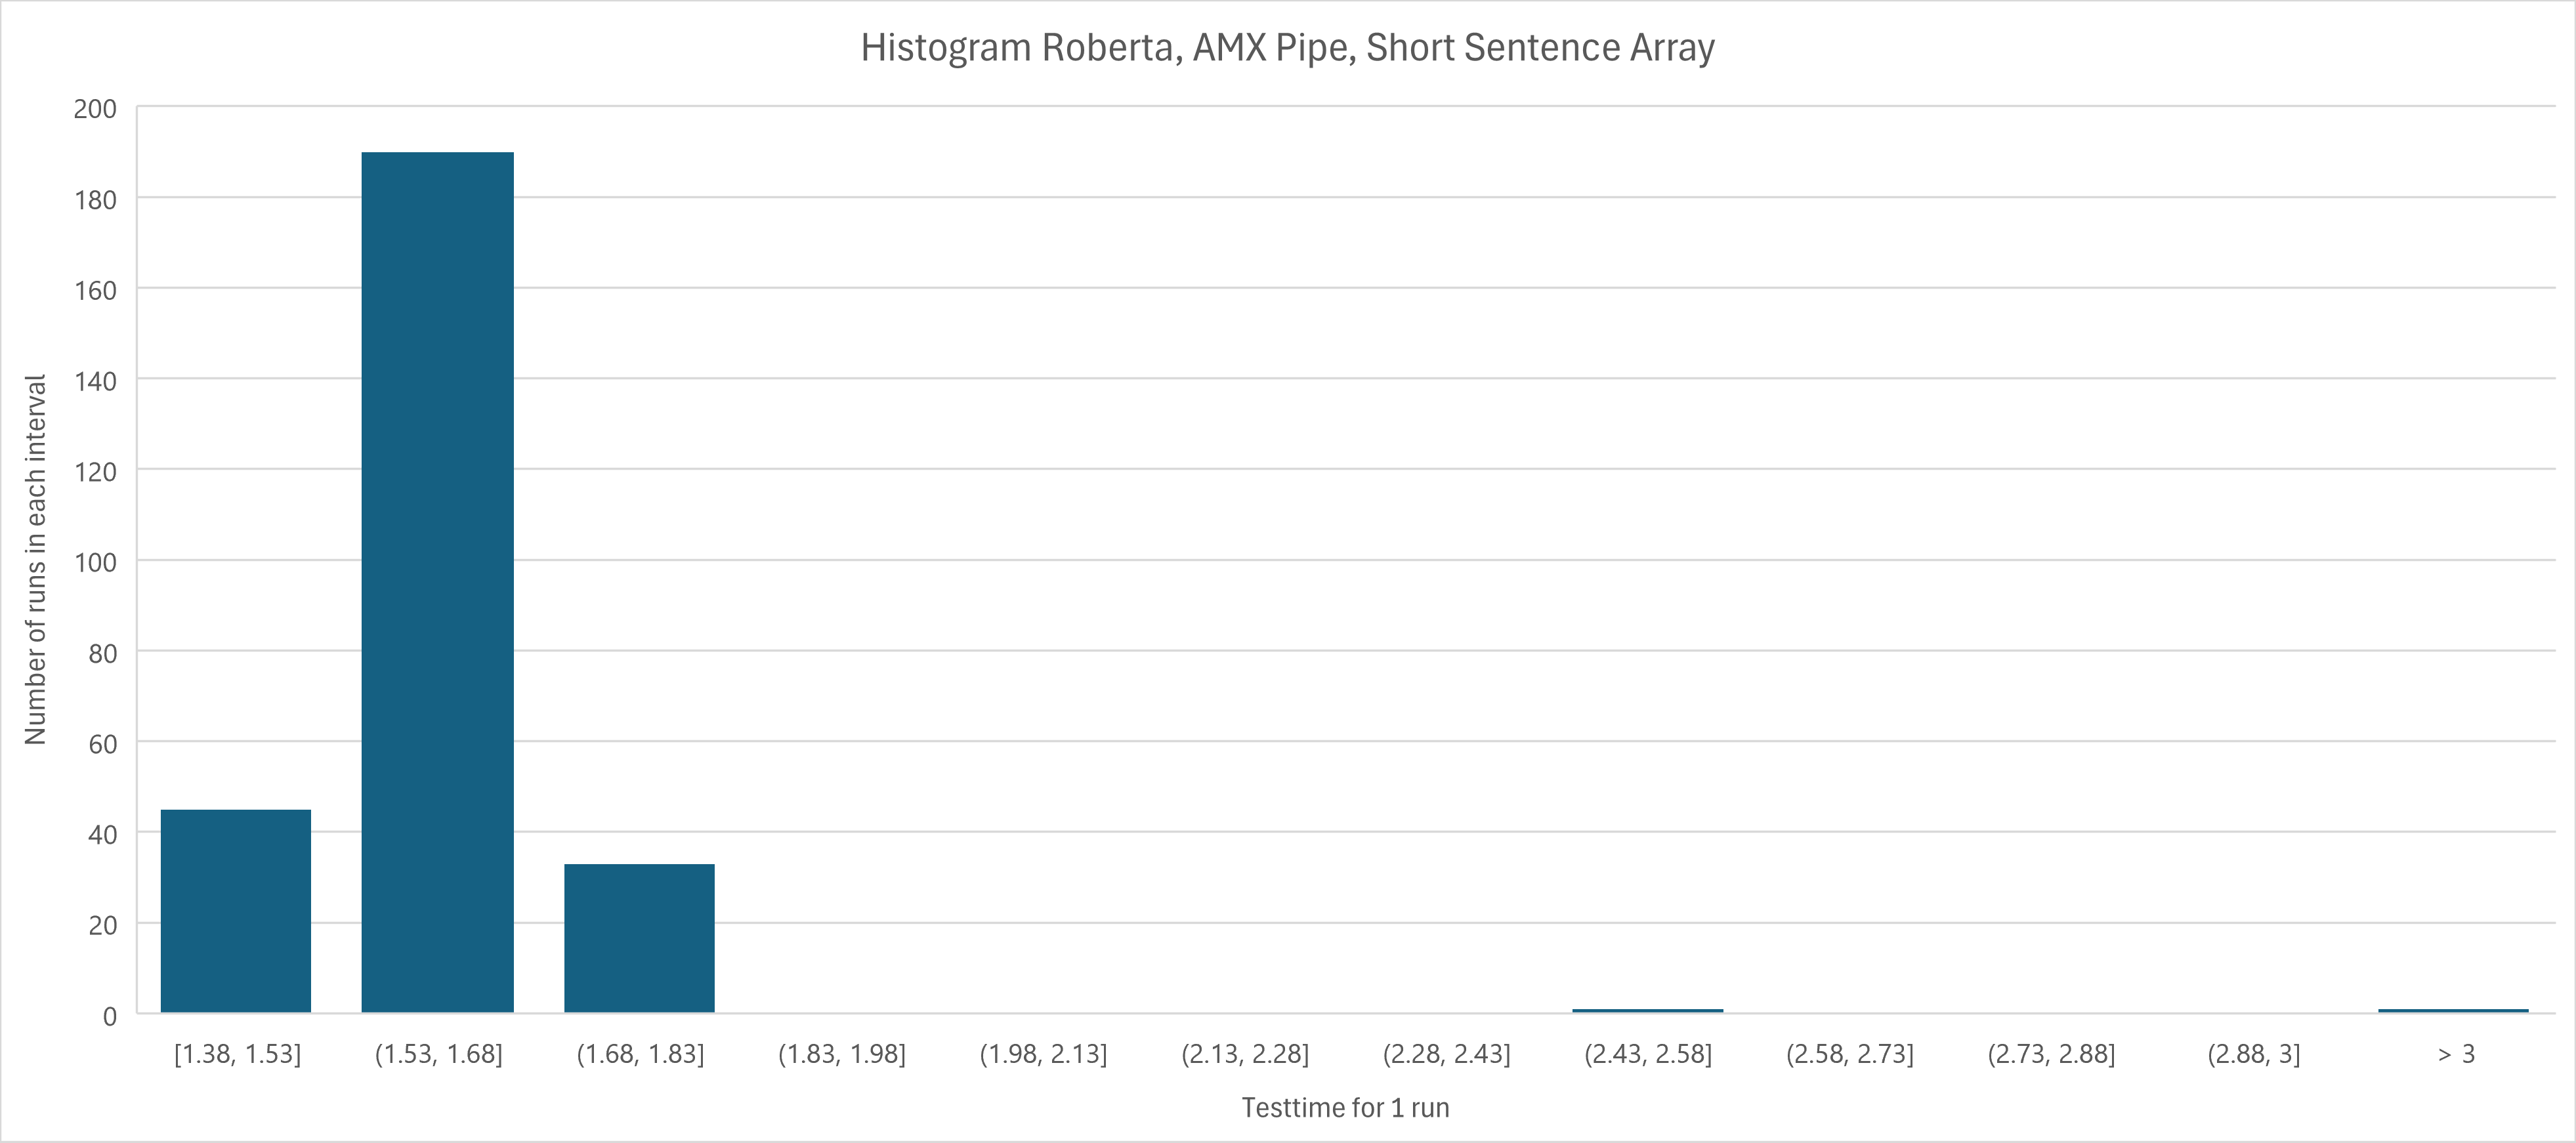
\includegraphics[width=\textwidth]{figures/Histogramm.png}
\caption{Shows the histogram of the short sentence array roBERTa AMX benchmark. The longest run to the right was over 6.4 seconds, but this would have made the diagram too big}
\label{fig:histogramm}
\end{figure}
A total of 2 out of 270 values were outliers but because some were so far outside the range 1.37s to 2.03s, the std dev was extremely high. Notably the longest run took 6.42 seconds almost 4 times as long as the mean. This one result increases the standard deviation from about 0.11 seconds to about 0.32 seconds. On the other hand the MAD only increases from about 0.03 to 0.04 seconds. The histogram clearly shows a clustering around about  1.65 seconds, which would not be appropriately represented by a standard deviation of 0.32 around the mean of 1.73 seconds. Each result was checked for significance using Student’s two-sample, two-tailed t-test with an alpha equal to 0.05, the most commonly used threshold. 

\subsection{Benchmark Results}
The initial testing was done using Ubuntu 22.04 on both the guest system as well as the host system. The system later on had stability issues, which is why testing was then moved to a different platform as well as using Ubuntu 23.10 on both host and guest. This section will first describe the results from testing on Ubuntu 22.04 and then later on describe the results from Ubuntu 23.10. The full benchmark results can be found in the files in the KIT library next to this thesis or in the Github repository.

\myparagraph{Ubuntu 22.04}

The Benchmark results using distilBERT-base-uncased show a small performance loss of 2\% from a TD VM to a Non-TD VM. The performance difference fluctuates between the non-TD VM being 3\% slower on the long sentence array transformer pipe to being 5\% faster on the long sentence AMX pipe. Half the benchmarks did not have a t-value that make them significant. These were run 90 instead of 30 times as previously discussed as the first run had unexpected results. The first run had the TD VM about 18\% faster on average, after running them twice more the gap closed overall but only one suite had the expected outcome of the Non-TD VM running faster. These results could not be replicated on a different platform. See \ref{app:bert} for the full results. The AMX variant was on average 29\% faster with the differences ranging from 19\% to 50\% faster.

The benchmark results using RoBERTa show a small performance loss of on average 1\% from a non-TD VM to a TD VM. The performance differs from about 5\% faster to 5\% slower. The absolute t-values range from 3.79 to 11.28. With 30 runs per test this results in p-values far below 0.01. All results except two were faster on non-TD VMs. The AMX accelerated pipe was faster on the TD VM on the short sentence array and long sentences. So while theses tests are statistically significant the difference in speed is not significant for real-world applications. AMX vs Non-AMX showed a speed increase of about 30\% in this benchmark, this is in line with the expected 1/3 speed increase.
\cref{fig:robertaUbuntu22.04} shows these miniscule differences quite well.
\begin{figure}
   \centering
       \includegraphics[width=.95\textwidth]{figures/Ubuntu22Roberta.png} 
 \caption{roberta-base inference times on Ubuntu 22.04}
 \label{fig:robertaUbuntu22.04}
\end{figure}


Both of the previous tests were done using an additional layer using a QEMU VM. Running the same benchmarks on the Host system directly averages an improvement of about 10\%. 
Due to the small margin between non-TD VMs and TD VM it was decided to test what disabling all TDX-related BIOS settings would have as an impact. This showed a significant speedup of on average 24\% using distillbert and 44\% using Roberta. The highest speed-up with 78\% was observed on the short-sentence array using Roberta. The difference was measurably slower using the AMX pipe with the distilbert TDX-enabled AMX pipe on the long-sentence being 5\% faster even. This difference was still inside the MAD, so could reasonably be explained with variations in testing. On average the non-AMX benchmarks were 53\% faster using distillbert and 71\% faster using Roberta. Figure \ref{fig:distillbertMADNONAMX} clearly shows the speed difference after disabling TDX in the BIOS. 
\begin{figure}
   \centering
       \includegraphics[width=.95\textwidth]{figures/distillbertMAD.png} 
 \caption{Distillbert Inference times on Ubuntu 22.04 without AMX}
 \label{fig:distillbertMADNONAMX}
\end{figure}
On the other hand Figure \ref{fig:distillbertMADAMX} shows no measurable speed difference after disabling TDX using the AMX-enabled Benchmarks. 
\begin{figure}
   \centering
       \includegraphics[width=.95\textwidth]{figures/distillbertMADAMX.png} 
 \caption{Distillbert Inference times on Ubuntu 22.04 using AMX}
 \label{fig:distillbertMADAMX}
\end{figure}
The AMX benchmarks were, using the geometric mean, similar in speed using distillbert, with a difference that was not statistically significant. The AMX benchmarks using Roberta were about 21\% faster. The overall speed-up was measurably faster than the initial observed AMX speedup, which indicates that this is not due to the omission of AMX in general but something different but having no speed-up using AMX with distillbert was an interesting result, which had no explainable reason. 

\myparagraph{Ubuntu 23.10}

All prior tests were done using Ubuntu 22.04 but due to the aforementioned stability issues a new platform with Ubuntu 23.10 was supplied by Intel. Rerunning the same tests using Ubuntu 23 the observed speed-up from a TD to TDX disabled diminished to just about 3\% with just TDX disabled and then an additional 3\% with memory-encryption disabled as well. These differences were small but the MAD on the measurements was even smaller, as can be seen in  \cref{fig:distillbertAMXUbuntu23}, so while these tests did not show large differences they appeared to be a lot more stable. 
\begin{figure}
   \centering
       \includegraphics[width=.95\textwidth]{figures/inferencedistillbertMADUbuntu23AMX.png} 
 \caption{Distillbert Inference times on Ubuntu 23 and Sapphire Rapid CPUs.Note: the apparent decrease in MAD is due to the logarithmic scale}
 \label{fig:distillbertAMXUbuntu23}
\end{figure}

A further examination was conducted on discernible execution time differences using a profiler on Ubuntu 23, but with just an eight percent speed difference, there was not much to observe. Minus the speed overhead of the profiler which was measured to be about 10 seconds, no matter the settings on the plattform, the execution took between 77 and 85 seconds, with the highest being TDX and memory encryption bypass enabled, which supposedly speeds up calculations. Some internal methods showed significant differences. The Intel Extension For Pytorch (IPEX) optimizer copy method saw timing increases of up to 400\%, this seems to be entirely due to activating TDX, as without TDX the timings were all within one percent of each other, enabling TDX without memory bypass increased this time by about 100\% and enabling bypass increases this a further 250\%. This method is called when AMX is enabled for the instruction set optimization. Total times for this IPEX optimization instruction can be seen in \ref{tab:IpexOpti}. The IPEX replacement method for linear transformation which takes most of the calculations shows small speed differences of about 5\% - which is about the same difference that was observed with the normal linear transformation method. The other methods all took about 5\% longer as well, which appears to be in line with the differences in memory access speed.
Having a look at the profiler results on the Azure cloud there are no clear results on overall speed but noticeably the IPEX copy and optimize instructions were once again measurably slower on the TD compared to a non-TD VM the optimization took about 20\% longer on the TD. This slow down is almost completely due to the time PyTorches clone function takes, which saw increases of around 1000\% in total and per call time. Memory encryption itself had close to no impact on the speed here. Neither did the Memory Encryption Bypass. Looking into the implementation of this function this is not expected. Clone creates shallow copies of a tensor, with the lower hierarchy memory being shared between the copies. With both the original and the copy being situated inside the TD, this is not a particularly demanding instruction. Its overhead should be similar in magnitude to the memory latency difference shown in \cref{tab:MemoryAccessSpeed}. Such a big overhead can be explained if a lot of context switching between encrypted and unencrypted memory has to be done, but this is not the case here.
\begin{table}
\centering
\resizebox{\textwidth}{!}{%
\begin{tabular}{ m{0.2\textwidth} m{0.2\textwidth} m{0.2\textwidth} m{0.2\textwidth} m{0.2\textwidth} m{0.2\textwidth}}
\toprule
& TD with ME Bypass & TD without ME Bypass & No-TD with ME & No-TD with ME Bypass & No Memory Encryption \\
\midrule
IPEX optimize total time & 1.21s & 0.597s & 0.28s & 0.278s & 0.284s \\
\midrule
PyTorch clone method & 1.01s & 0.397s & 0.079s & 0.077s & 0.077s \\
\bottomrule
\end{tabular}
}
\caption{Comparison of different timings of IPEX optimization method}
\label{tab:IpexOpti}
\end{table}


\subsection{Benchmarking TDX parts}

As stated in the previous section there were significant speed differences between having TDX enabled and disabled in the Bios but basically none when TDX was enabled in the Bios but disabled in the VM. Further investigations into what causes these speed-ups were necessary. As stated in \ref{sec:tdxBuildingBlocks} there were essentially two functionalities that could theoretically be tested independently from TDX, which could have a performance impact:
\begin{itemize}
    \item Total Memory Encryption 
    \item Intel VT, virtualization features
\end{itemize}
Intel SGX is only used for attestation purposes and thus does not have a performance impact. From TME and VT only TME was successfully tested as disabling VT prevented the system from booting.
For Total Memory Encryption, TDX and SGX were disabled, while Intel VT remained turned on. Stream \cite{mccalpin_memory_1995} and "PerformanceTest" \url{https://www.passmark.com/products/pt_linux/index.php} were used for benchmarking. Stream is the de facto standard for memory speed testing and PerformanceTest is a commonly used proprietary tool used to compare memory access speed. Using PerformanceTest there were small but measurable differences in speed of about 2.5\% for reading speed. The Writing speed remained within 1\% of each other. \cref{tab:MemoryAccessSpeed} shows the differences in more detail. The latency increased nearly 4.5\%.
\begin{table}
\centering
\resizebox{\textwidth}{!}{%
\begin{tabular}{ m{0.37\textwidth} m{0.25\textwidth} m{0.25\textwidth} m{0.13\textwidth}}
\toprule
Memory Benchmark Type & Memory encryption activated & Memory encryption deactivated & Difference \\
\midrule
Memory Allocation MB/s & 32445.11 & 33258.94 & 2.5\% \\
\midrule
Memory Read Cached MB/s & 27683.36 & 28148.14 & 1.6\% \\
\midrule
Memory Read Uncached MB/s & 10879.98 & 11123.77 & 2.2\% \\
\midrule
Memory Write Medium MB/s & 9592.82 & 9549.92 & -0.4\% \\
\midrule
Memory Write Threaded MB/s & 400550.9 & 411297.5 & 2.6\% \\
\midrule
Memory Latency ns & 64.3 & 61.4 & -4.5\% \\
\bottomrule
\end{tabular}
}
\caption{Results of Performancetests memory benchmark}
\label{tab:MemoryAccessSpeed}
\end{table}

With Stream, everything was tested disabled, just Memory Encryption enabled, and TDX completely enabled, and all three were within two percent of one another, with the encrypted memory being slightly faster than the other two. These results are most likely due to background noise of the system.

\begin{table}[]
    \centering
    \resizebox{\textwidth}{!}{%
    \begin{tabular}{m{0.2\textwidth} m{0.2\textwidth} m{0.2\textwidth} m{0.2\textwidth} m{0.2\textwidth} m{0.2\textwidth}}
    \hline
        Function & Best Rate MB/s Encrypted & Best Rate MB/s TDX enabled & Best Rate MB/s unencrypted & Best Rate Legacy VM MB/s & Best Rate TD MB/s \\ \hline
        Copy: & 292927.7 & 296714.7 & 299686.3 & 228281.2 & 209348.5979 \\ \hline
        Scale: & 291833.5 & 296603.3 & 298131.2 & 225828 & 206950.9938 \\ \hline
        Add: & 324643.9 & 318742.3 & 331304.6 & 250686.5 & 221401.8875 \\ \hline
        Triad: & 315635.1 & 329435.5 & 334132 & 232469.4 & 225711.5192 \\ \hline
        Normalized Geometric Mean & 1.418 & 1.437 & 1.462 & 1.085 & 1.000 \\ \hline
    \end{tabular}
    }
    \caption{Comparison of Memory Access speed using STREAM for various Non-VM settings as well as legacy VMs and TD}
\end{table}



\subsection{Security Attestation}

Attestation was not implemented or usable on the Intel Developer Cloud. Verifying usage of TDX was thus relying on the Linux Kernel itself as well as BIOS settings made by the user via an SSH connection. Without attestation the security benefits were theoretically not given. This was accepted as having bare-metal access meant being able to verify TDX activation directly and this hardware was only used for benchmarking.


\subsection{Performance Summary}
\label{Perf_EVal}

The initial testing on Ubuntu 22.04 showed the surprising result of having basically no slowdown or even a speedup when using TDX compared to a normal VM, while having TDX enabled in the BIOS. This results changed drastically when disabling TDX in the BIOS to about 30\% faster execution compared to the TD. These results persisted upon rerunning the tests on the same platform, although having the TD be faster on a different platform was not replicable. These results did not persist upon switching the platform, where the results were more inline with the expected five to ten percent difference, when using memory encryption. TD and non-TD VM, with the TDX being enabled stayed close to each other, which shows that there are basically no software-related slowdowns. A single method, which was necessary for the Intel AMX improved instructions, which only creates shallow copies showed significant slowdown of up to 1000\%. These were reproducible but it is unclear how they came to be. Overall the usage of a TD reduces inference speed by about ten percent, with most of this being due to the decreased memory speed, coming from the memory encryption. Using a non-TD on TDX enabled hardware offers no performance benefits. Additionally hosting a VM using QEMU decreases inference speed by about 30\% on its own, meaning the difference between TDX enabled and TDX disabled is a lot smaller than the difference between executing directly on the host vs inside a QEMU VM.



